\chapter{Werking cartridge}
\chapterpreamble

\section{Broncode}

In dit hoofdstuk wordt de werking van de \product uitgelegd. Ondanks dat er redelijk wat details besproken worden blijft deze uitleg relatief oppervlakkig daar een gedetailleerde uitleg een veelvoud aan pagina's zou behoeven. De beschrijvingen in dit hoofdstuk moeten vooral als conceptueel beschouwd worden en voor meer details wordt aangeraden om de originele schema's en broncode op de Github pagina te raadplegen.\\
\url{https://github.com/ifilot/p2000t-sdcard/}

%
%
%
\section{Printplaat}

Het ``hart'' van de \product is de printplaat in de \sleuf{2} cartridge. Een schematische afbeelding van deze printplaat en diens componenten staat afgebeeld in \cref{fig:pcb-design}. Voor het schakelschema, zie pagina \pageref{sec:schematic-cartridge2}.

\begin{figure}[h!]
    \centering
    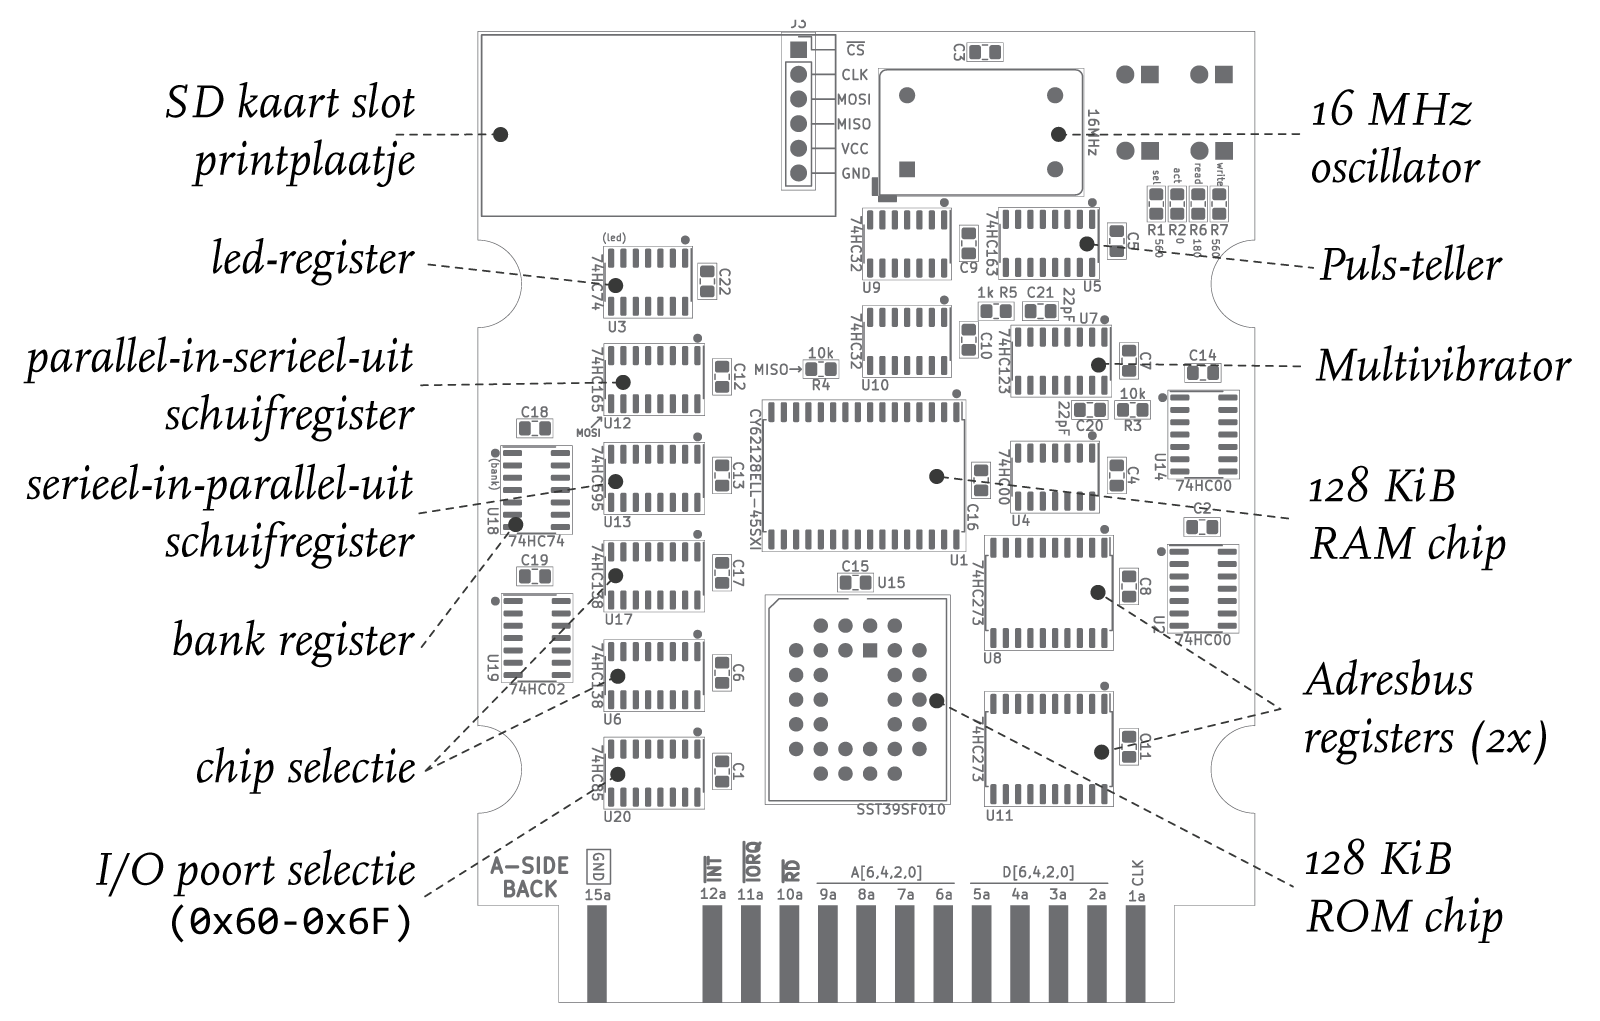
\includegraphics[width=0.99\textwidth]{img/pcb-design}
    \caption{Schematische weergave van de achterzijde van de printplaat en de functionaliteit van de diverse chips.}
    \label{fig:pcb-design}
\end{figure}

De verbinding tussen de \pkb{P2000T} en de SD-kaart is een seriële verbinding conform het SPI protocol. In dit protocol gebeurt de data-overdracht tussen twee apparaten simultaan. Om een byte aan data uit te lezen vanaf de SD-kaart moet er ook eerst een byte ingaan. Dit gebeurt via twee schuifregisters: een parallel-in-serieel-uit (PISU) en een serieel-uit-parallel-in (SUPI) schuifregister.\footnote{In het Engels zijn deze afkortingen PISO en SIPO.} Middels een enkele instructie kan de \pkb{P2000T} een byte aan data wegschrijven in het PISU schuifregister. Vervolgens wordt er gecontroleerd 8 pulsen op 8 MHz aangeslagen om de data vanuit de PISU naar de SD-kaart weg te schrijven. Simultaan worden dan ook 8 bits aan data (1 byte) ontvangen in de andere SIPU register welke wederom middels een enkele operatie door de \pkb{P2000T} uitgelezen kan worden. De pulsen worden gegenereerd door de 16 MHz oscillator welke middels de puls-teller door twee wordt gedeeld om een 8 MHz signaal te geven. De multivibrator zorgt ervoor dat deze pulse-generator niet vroegtijdig voor een tweede keer geactiveerd kan worden. Het grote voordeel van deze opstelling is dat elke machine-instructie van de \pkb{P2000T} optimaal benut kan worden en dat er geen vertraging optreedt bij de parallel-naar-serieel conversie daar deze volledig in hardware verloopt.

De verscheidene componenten op de \sleuf{2} cartridge zijn allen aangesloten op de onderste byte van de adresbus (\pkb{A0-A7}) en de databus (\pkb{D0-D7}). Ze kunnen benaderd worden via I/O poorten \pkb{0x60-0x6F}. Afhankelijk van de specifieke I/O waarde wordt slecht één van de chips geactiveerd.

Naast het SD-kaartje bevat de \sleuf{2} cartridge ook een 128 KiB RAM en 128 KiB ROM chip. Omdat enkel de onderste byte van de adresbus toegankelijk is in \sleuf{2}, moet er gebruikt gemaakt worden van additionele registers om het volledige geheugen op deze chips aan te kunnen spreken. De twee adresbus registers worden gedeeld door de ROM en RAM chip en kunnen tezamen 64 KiB geheugen adresseren. Middels een 2 x 1-bit bank register kan hiermee ofwel de onderste of de bovenste 64 KiB van de 128 KiB benaderd worden. Het bank register wordt niet door de RAM en ROM chips gedeeld; elke chip heeft zijn eigen 1-bit register.

Tenslotte heeft de \sleuf{2} cartridge vier LED-lampjes. De bovenste twee LED-lampjes worden puur hardwarematige aangestuurd. Wanneer de SD-kaart geactiveerd is zal het gele lampje branden. Bij data-overdracht zal het ambergekleurde lampje branden. De onderste twee LEDjes worden softwarematig aangestuurd middels een 2 x 1-bit register.

%
%
%
\section{Geheugenmodel}
\label{sec:memory-model}

De \product gaat uit van verschillende geheugenmodellen van de \pkb{P2000T}. Een overzicht van deze modellen is weergegeven in \cref{fig:memory-models}. De meest basale variant omvat de zogehete ``kale'' \pkb{P2000T} welke 16 KiB aan geheugen heeft. Dit is de meest beperkende configuratie en bepaalt feitelijk de bovenste limiet van de grootte van de firmware. In deze configuratie plaatst de monitor de top van de stack op \pkb{0x9FFF}. De programmatuur van de \product wordt geplaatst op \pkb{0x7000-0x9CFF} en mag dus maximaal $11520$ bytes beslaan.

\begin{figure}[h!]
    \centering
    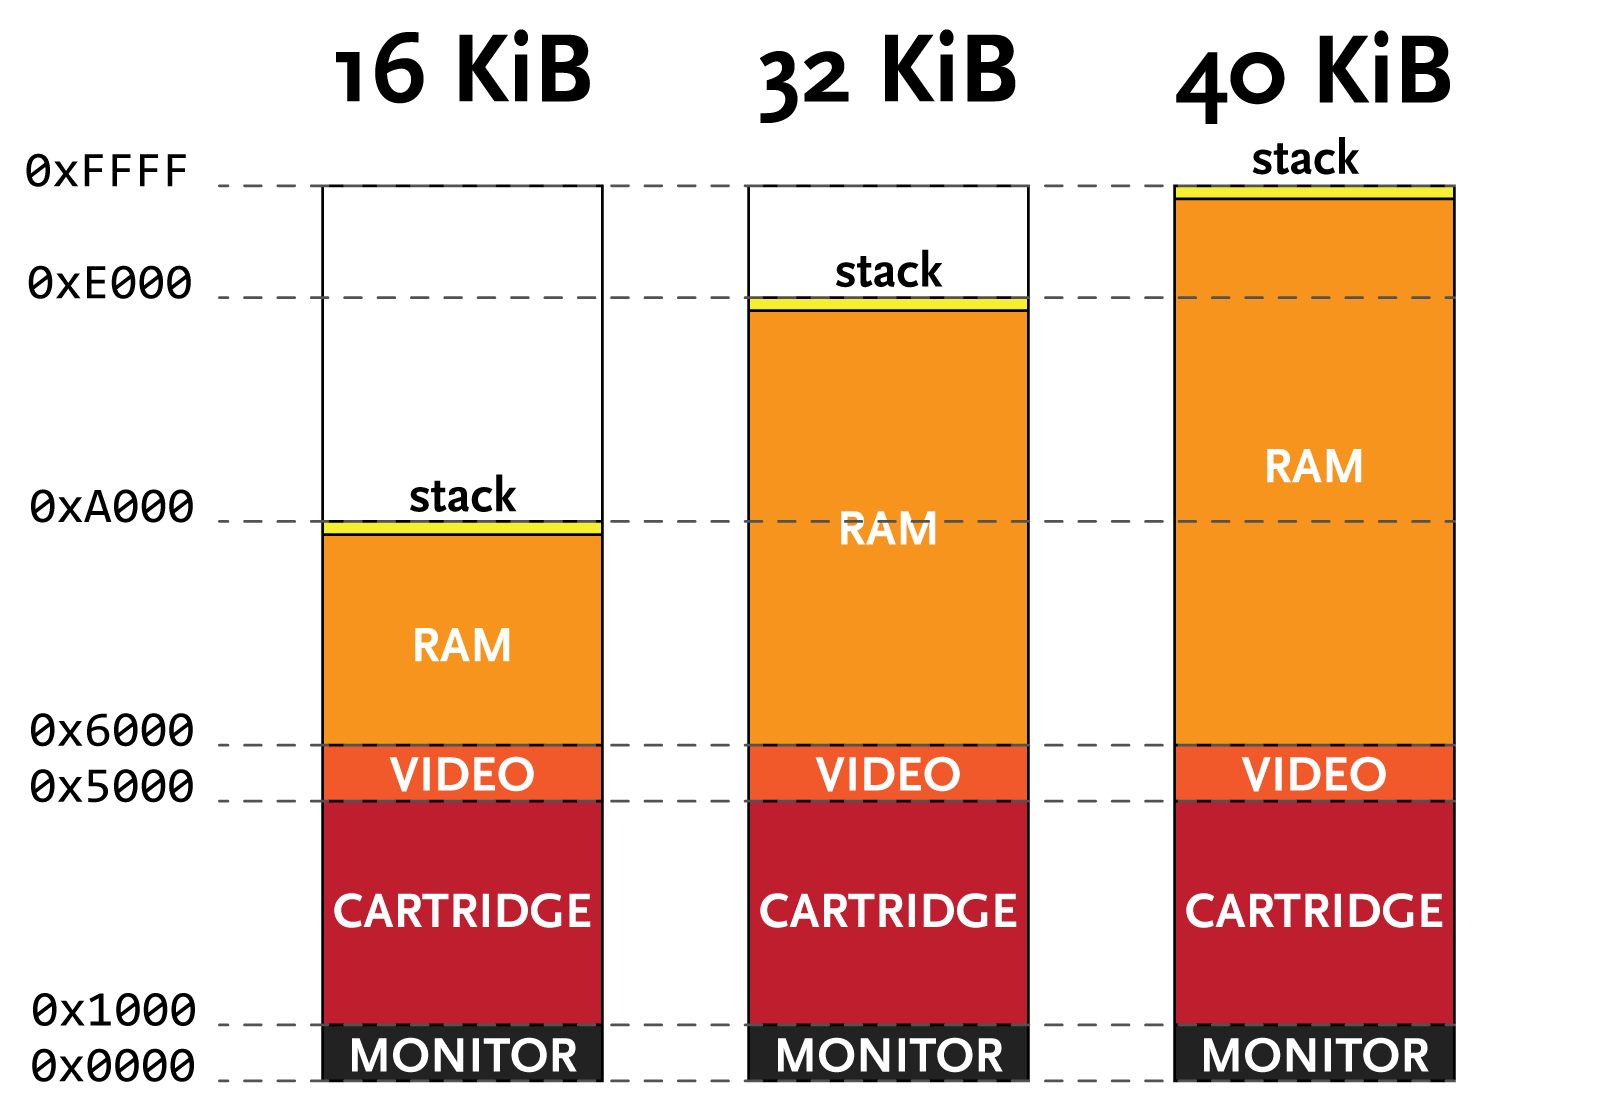
\includegraphics[width=0.99\textwidth]{img/memory_models.png}
    \caption{Geheugenmodellen van de \pkb{P2000T}.}
    \label{fig:memory-models}
\end{figure}

In de iets uitgebreidere scenario heeft de \pkb{P2000T} een 16 KiB geheugenuitbreiding en in totaal dus 32 KiB geheugen. Hierdoor wordt het geheugenbereik \pkb{0xA000-0xDFFF} beschikbaar en plaatst de monitor de top van de stack op \pkb{0xDFFF}. De extra 16 KiB aan geheugen kunnen gebruikt worden om \pkb{PRG} programma's op te starten. Deze stand-alone programma's worden geplaatst op \pkb{0xA000-0xDCFF} en hebben hun eigen stack (van maximaal 512 bytes) waarvan de top geplaatst is op \pkb{0xDEFF}. Deze positie zorgt ervoor dat de programma's niet interfereren met de \pkb{BASIC} stack.

In het meest uitgebreide scenario is ook het geheugenbereik \pkb{0xE000-0xFFFF} en wordt de top van de \pkb{BASIC} stack op \pkb{0xFFFF} geplaatst. Veelal beschikt de \pkb{P2000T} dan ook over ``bank switching'' waarbij het bovenste 8 KiB geheugenblok uitgewisseld kan worden voor een ander blok om zo nog meer geheugen aan te kunnen spreken. \pkb{PRG} programma's die gebruik willen maken van \pkb{0xE000-0xFFFF} en de mogelijkheid tot bank switching moeten zorgdragen dat deze operaties niet interfereren met de \pkb{BASIC} stack. Dit kan bijvoorbeeld door de bank met de \pkb{BASIC} stack eerst uit te wisselen voor een andere bank (of meer).

%
%
%
\section{Opstartprocedure}

Om \pkb{CAS} bestanden in te kunnen laden en af te spelen heeft de \product een \pkb{BASIC} omgeving nodig. Om die reden moeten de \pkb{BASIC} routines beschikbaar zijn in het geheugenbereik \pkb{0x1000-0x4FFF}. Omdat de \pkb{BASIC} cartridge niet volledig gevuld is, is er nog plaats over om een reeks aan (assembly) routines toe te voegen vanaf \pkb{0x4EC7}. Hier worden de routines geplaatst om de ROM chip op de \sleuf{2} uit te kunnen lezen en de firmware te kopiëren naar het interne RAM geheugen van de \pkb{P2000T}. Normaal gesproken wordt tijdens de \pkb{BASIC} boot op \pkb{0x1F71} een oproep gedaan naar adres \pkb{0x1056}, dat een sprong naar adres \pkb{0x1F5A} bevat. Deze oproep wordt gekaapt door de adres-pointer te veranderen op \pkb{0x1057-0x1058} naar \pkb{0x4EE0}, waar de inlaad-routines staan.

\begin{lstlisting}[caption=Vector tabel in BASIC]
...
jp $1548               ;$1053
jp $1f5a               ;$1056
jp $174f               ;$1059
...
\end{lstlisting}

\begin{lstlisting}[caption=Aangepaste vector tabel in BASIC]
...
jp $1548               ;$1053
jp $4ee0               ;$1056
jp $174f               ;$1059
...
\end{lstlisting}

Het kleine stukje code dat wordt ingevoegd op \pkb{0x4EE0} slaat tevens de waarde \pkb{0x55} op op het geheugenadres \pkb{0x6150} (dat vrij is om te gebruiken). Wanneer deze waarde aanwezig is, wordt een andere gekaapte geheugenroutine geactiveerd. Deze routine is vrij klein en bevindt zich op \pkb{0x4CE7}. Hier wordt gecontroleerd of geheugenadres \pkb{0x6150} de waarde \pkb{0x55} bevat, en indien zo, dan wordt een sprong gemaakt naar \pkb{0x6151} waar een aangepaste pointer geplaatst kan worden naar elk gewenst stukje code dat moet worden uitgevoerd.

Samengevat, met deze aanpassingen kan tijdens de \pkb{BASIC} boot procedure het proces omgeleid worden waardoor de firmware ingeladen wordt in het interne geheugen en opgestart wordt. Voor de exacte details kan het beste gekeken worden naar de originele broncode welke gevonden kan worden middels onderstaande link:\\
\url{https://github.com/ifilot/p2000t-sdcard/tree/master/basicmod}.

%
%
%
\section{SD-kaart}

De firmware probeert verbinding te maken met de SD-kaart en de eerste partitie op die kaart te benaderen. De \product kan enkel verbinding maken met SD-kaarten van het type SDHC welke geformatteerd moeten zijn met een FAT32 bestandssysteem. Voor het communiceren met de SD-kaart wordt gebruikt gemaakt van een protocol dat uitgaat van 6-byte instructies, welke beschreven staan in het document ``SD Card Physical Specification''.\footnote{Men kan dit document het beste vinden door deze term in te voeren in een zoekmachine.}

Om de SD-kaart in te lezen worden eerst 96 pulsen gestuurd om deze te laten ontwaken. Middels \cmd{0} wordt de kaart gereset hetgeen gevolgd wordt door \cmd{8}. Vervolgens wordt herhaaldelijk \pkb{CMD55 + ACMD41} gestuurd totdat de SD-kaart respondeert met de waarde \pkb{0x00}. Tenslotte wordt \cmd{58} gestuurd waarna de SD-kaart klaar is om lees- of schrijf-instructies te ontvangen middels \cmd{17} en \cmd{24}. Zie \cref{fig:sd-card-protocol} voor een diagrammatische weergave van het protocol.

\begin{figure}[h!]
    \centering
    \tikzstyle{block} = [draw, fill=white, rectangle, 
    minimum height=3em, minimum width=6em, rounded corners]

    \begin{tikzpicture}[auto, node distance=2.5cm,>=latex']
        \node [draw, circle, fill=primarycol] (start) {\color{white}START};
        \node [block, below of=start] (cmd0) {\ttfamily CMD0};
        \node [block, below of=cmd0] (cmd8) {\ttfamily CMD8};
        \node [block, below of=cmd8] (acmd41) {\ttfamily CMD55 + ACMD41};
        \node [draw, diamond, below of=acmd41] (lees) {Lees \ttfamily 0xFF\normalfont ?};
        \node [block, below of=lees] (cmd58) {\ttfamily CMD58};
        \node [draw, circle, below of=cmd58, fill=primarycol] (stop) {\color{white}ACTIEF};
        \node [block, right of=stop] (cmd17) {\ttfamily CMD17};
        \node [block, left of=stop] (cmd24) {\ttfamily CMD24};
    
        \coordinate [right=0cm and 2cm of lees] (path) {};
        \coordinate [above=1cm of cmd17] (cmd17t) {};
        \coordinate [above=1cm of cmd24] (cmd24t) {};
    
        \draw [->] (start) -- (cmd0);
        \draw [->] (cmd0) -- (cmd8);
        \draw [->] (cmd8) -- (acmd41);
        \draw [->] (acmd41) -- (lees);
        \draw [->] (lees) -- node {ja} (cmd58);
        \draw [-] (lees) -- (path);
        \draw [->] (path) |- node [near end] {nee} (acmd41);
        \draw [->] (cmd58) -- (stop);
        \draw [->] (stop) -- (cmd17);
        \draw [->] (stop) -- (cmd24);
        \draw [->] (cmd17) -- (cmd17t) -| (stop);
        \draw [->] (cmd24) -- (cmd24t) -| (stop);
        
    
    \end{tikzpicture}
    \caption{Diagram van het communicatieprotocol met de SD-kaart. Middels een serie van commando's wordt de SD-kaart in een staat geprepareerd waardoor middels \cmd{17} en \cmd{24} een sector (512 bytes) uitgelezen, respectievelijk weggeschreven kan worden.}
    \label{fig:sd-card-protocol}
\end{figure}

In onderstaande lijst staat welk commando welke operaties uitvoeren op de SD-kaart.

\begin{itemize}
    \item \cmd{0}: Reset de SD-kaart.
    \item \cmd{8}: Controleert op welke spanningen de SD-kaart kan opereren.
    \item \cmd{41}: Activeert het initialisatie-proces van de SD-kaart. Omdat dit even duurt, wordt herhaaldelijk getoetst of de SD-kaart gereed is.
    \item \cmd{58}: Lees het OCR (operation condition register) uit.
    \item \cmd{17}: Lees een sector.
    \item \cmd{24}: Schrijf een sector.
\end{itemize}

%
%
%
\section{FAT32}

De communicatie met de SD-kaart betreft enkel ruwe data-overdracht en is onafhankelijk van het bestandssysteem dat op de SD-kaart staat. Om bestanden te kunnen vinden moet de data geïnterpreteerd worden. De \product gaat ervan uit dat de SD-kaart geformatteerd is met een FAT32 bestandssysteem welke relatief makkelijk te gebruiken is. Elke FAT32 partitie, zie \cref{fig:fat32-partition} bestaat uit een sector met partitie-informatie (VOLUME ID), gevolgd door enkele gereserveerde sectoren, daarna twee FATs (file allocation tables) en tenslotte een hele reeks clusters.

\begin{figure}[h!]
    \centering
    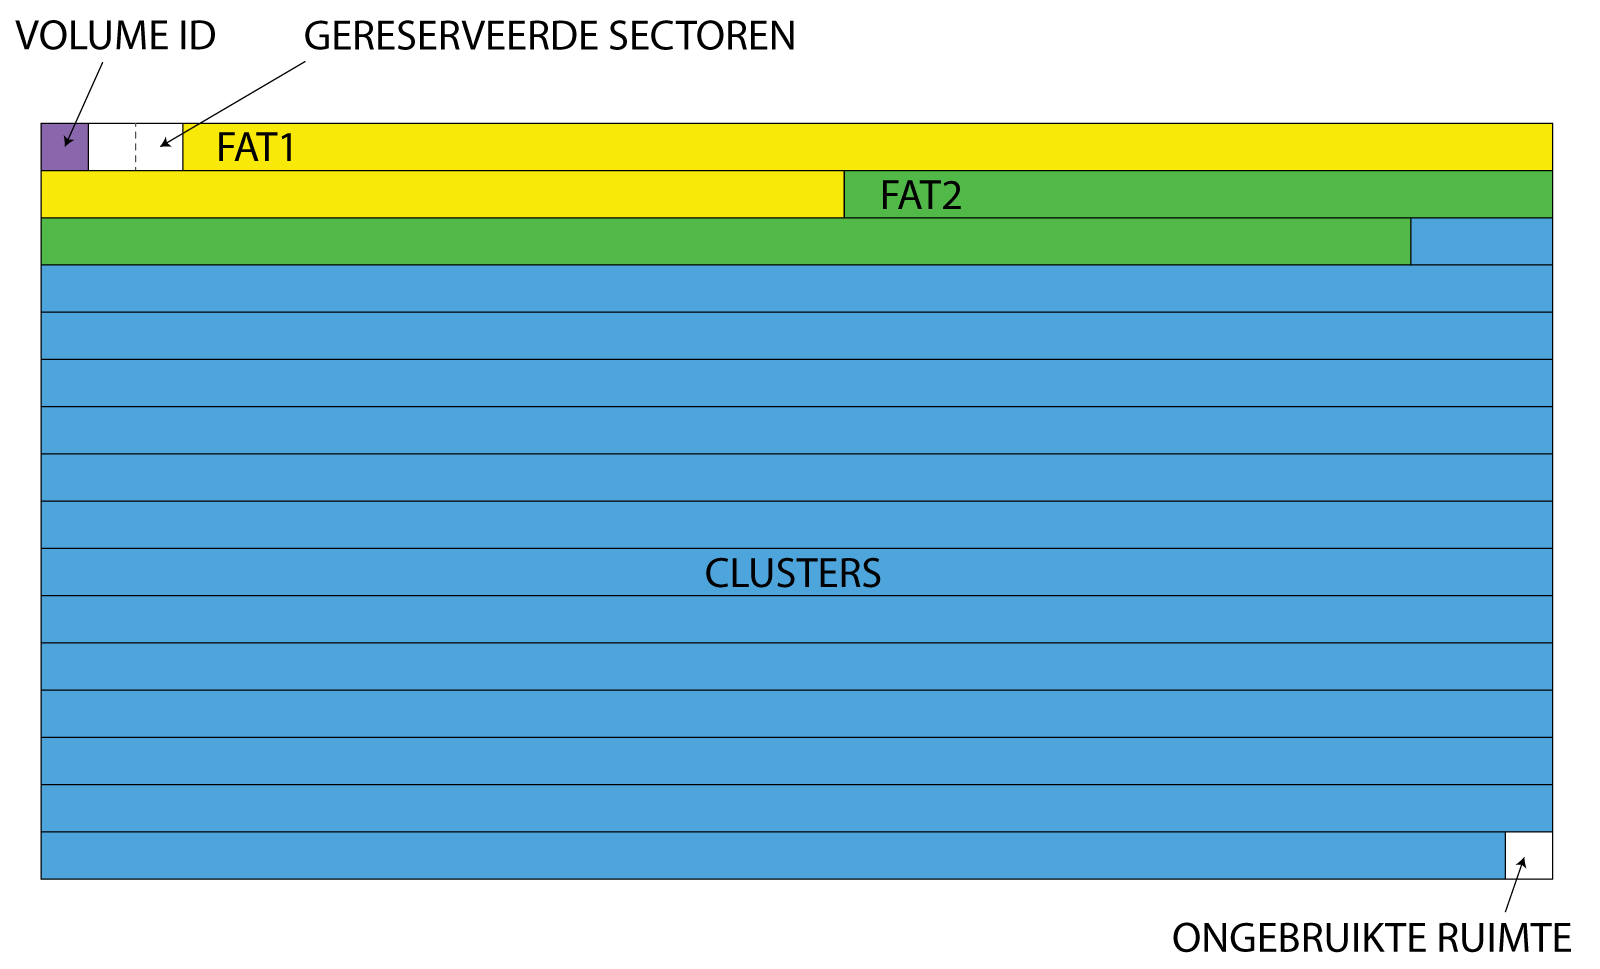
\includegraphics[width=0.70\textwidth]{img/fat32-partitie.png}
    \caption{Partitie-indeling van een FAT32 bestandssysteem.}
    \label{fig:fat32-partition}
\end{figure}

Bij het inlezen van een SD-kaart wordt eerst de boot-sector gelezen (\cref{fig:boot-sector}). Dat is de eerste sector op het SD-kaartje en deze geeft per partitie aan waar dat de partitie zich bevindt. Deze sector heeft aan het einde de 16-bit signatuur \pkb{0x55AA} welke gebruikt kan worden ter controle of deze sector correct is uitgelezen.

\begin{figure}[h!]
    \begin{subfigure}[t]{0.3\textwidth}
        \centering
        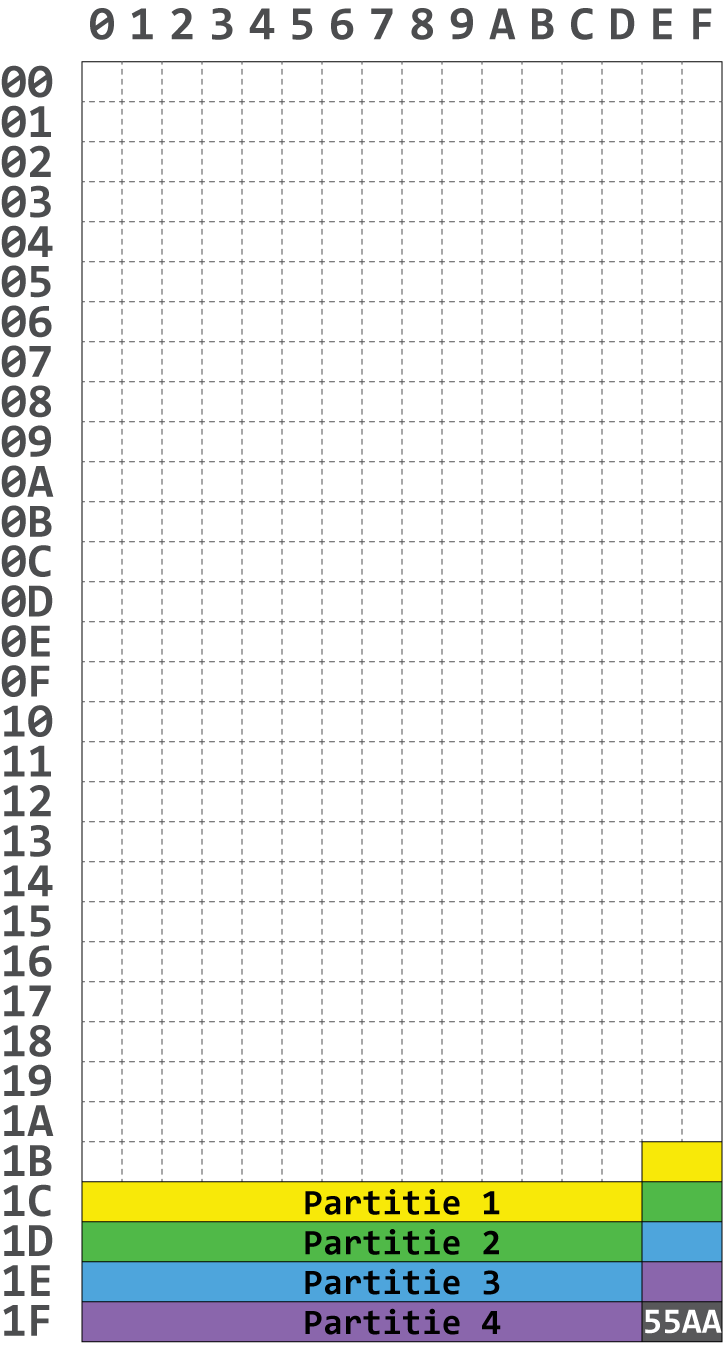
\includegraphics[width=0.95\textwidth]{img/boot-sector.png}
        \caption{Boot-sector}
        \label{fig:boot-sector}
    \end{subfigure}%
    ~ 
    \begin{subfigure}[t]{0.7\textwidth}
        \centering
        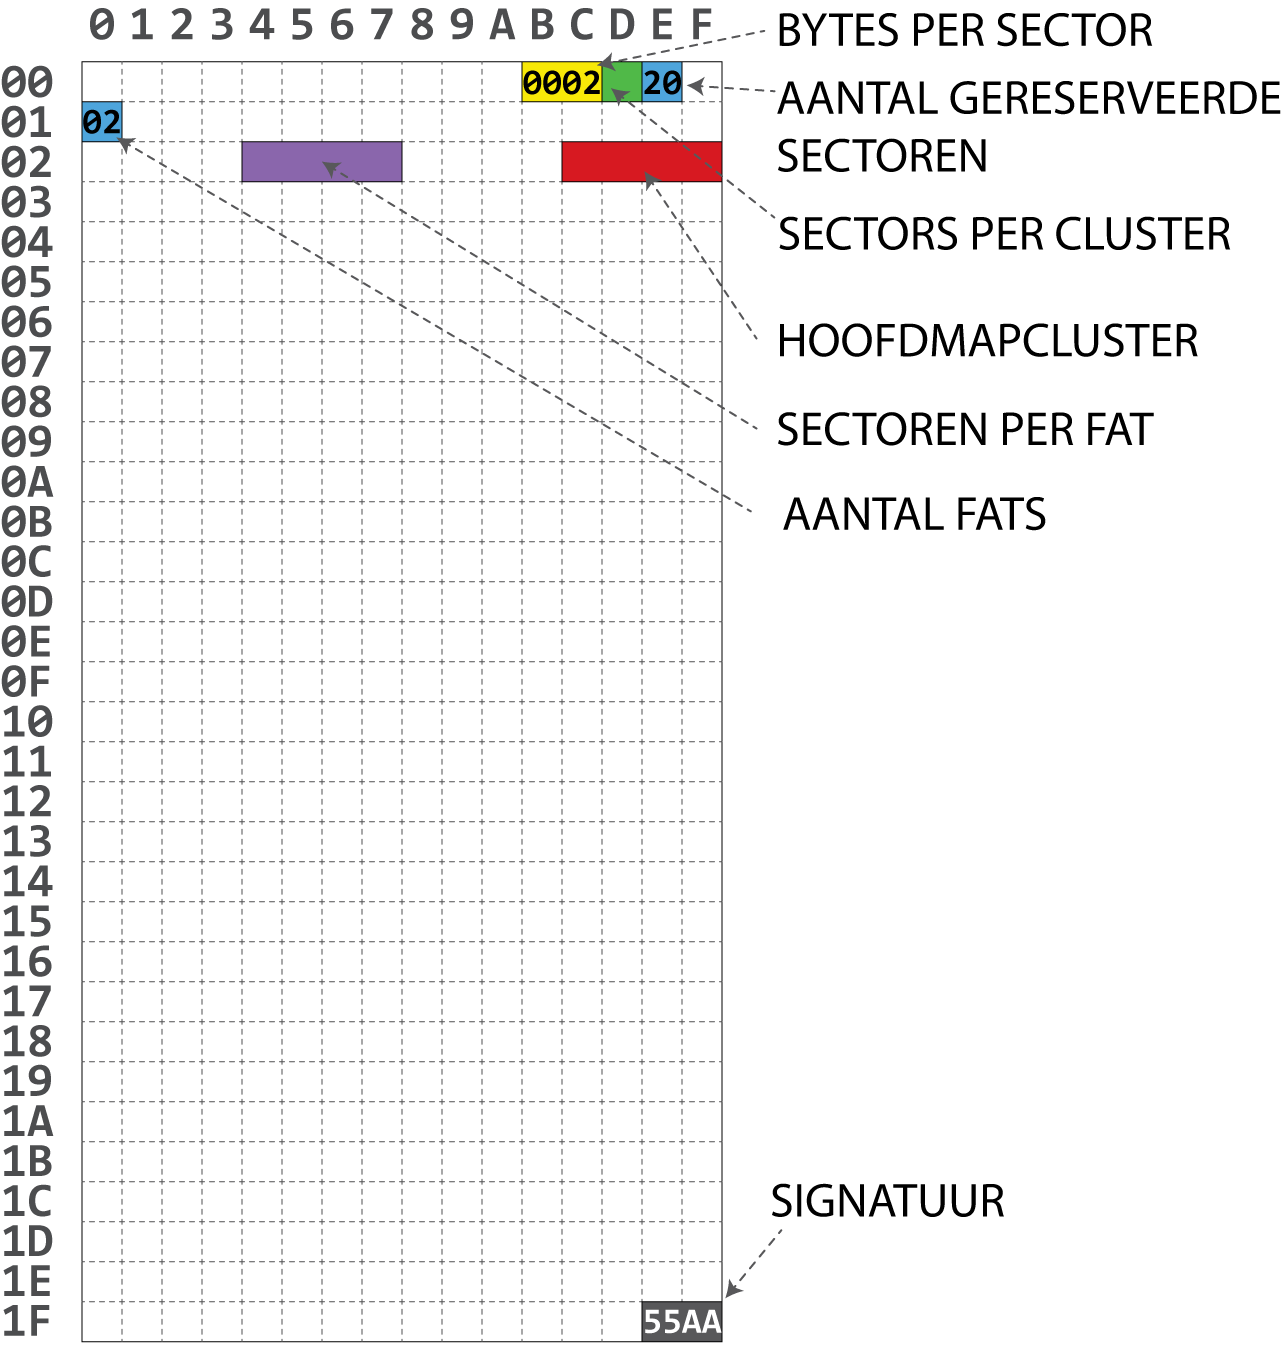
\includegraphics[width=0.95\textwidth]{img/volume-id.png}
        \caption{Eerste sector van een partitie}
        \label{fig:volume-id}
    \end{subfigure}
    \caption{(a) Boot-sector van de SD-kaart en (b) eerste sector van een partitie met aanduiding van de relevante partitiegevens.}
\end{figure}

Op basis van de boot-sector kan de eerste sector van een partitie gevonden worden (\cref{fig:volume-id}). Op deze sector staat een reeks aan belangrijke gegevens om de partitie uit te kunnen lezen. Sommige van deze gegevens staan in principe altijd vast voor FAT32 bestandssystemen, zoals het aantal bytes per sector (512 bytes), het aantal gereserveerde sectoren (20) en het aantal FATs (2). Andere zaken hangen af van de formatteerinstellingen. Zo kan tijdens het formatteren met een FAT32 bestandssysteem de clustergrootte gekozen worden, welke het aantal sectoren per cluster en het aantal sectoren per FAT bepaald. Op basis van het aantal sectoren per FAT en het aantal sectoren per cluster kan de totale capaciteit van de partitie uitgerekend worden. Ook staat in de eerste sector van de partitie het clusteradres van de hoofdmap. Dit adres bepaalt waar we moeten beginnen met lezen wanneer we het bestandssysteem willen navigeren.

\begin{figure}[h!]
    \begin{subfigure}[t]{0.6\textwidth}
        \centering
        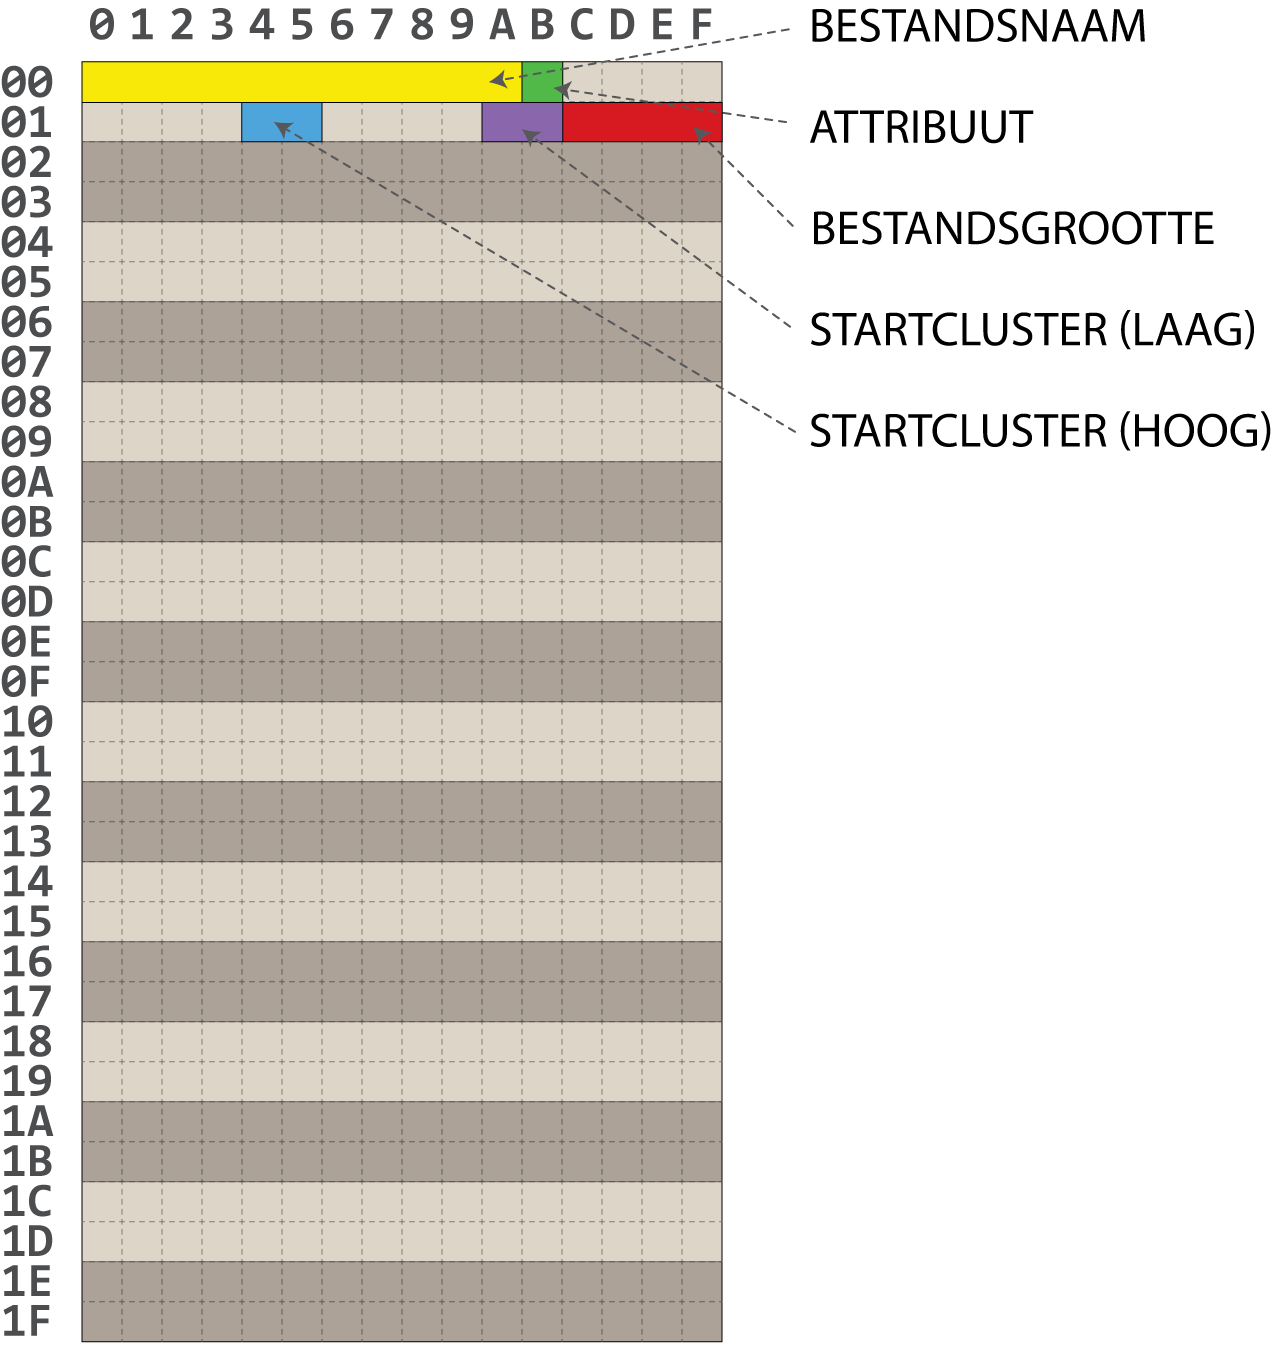
\includegraphics[width=0.95\textwidth]{img/folder-cluster.png}
        \caption{Folder sector.}
        \label{fig:folder-cluster}
    \end{subfigure}%
    ~ 
    \begin{subfigure}[t]{0.4\textwidth}
        \centering
        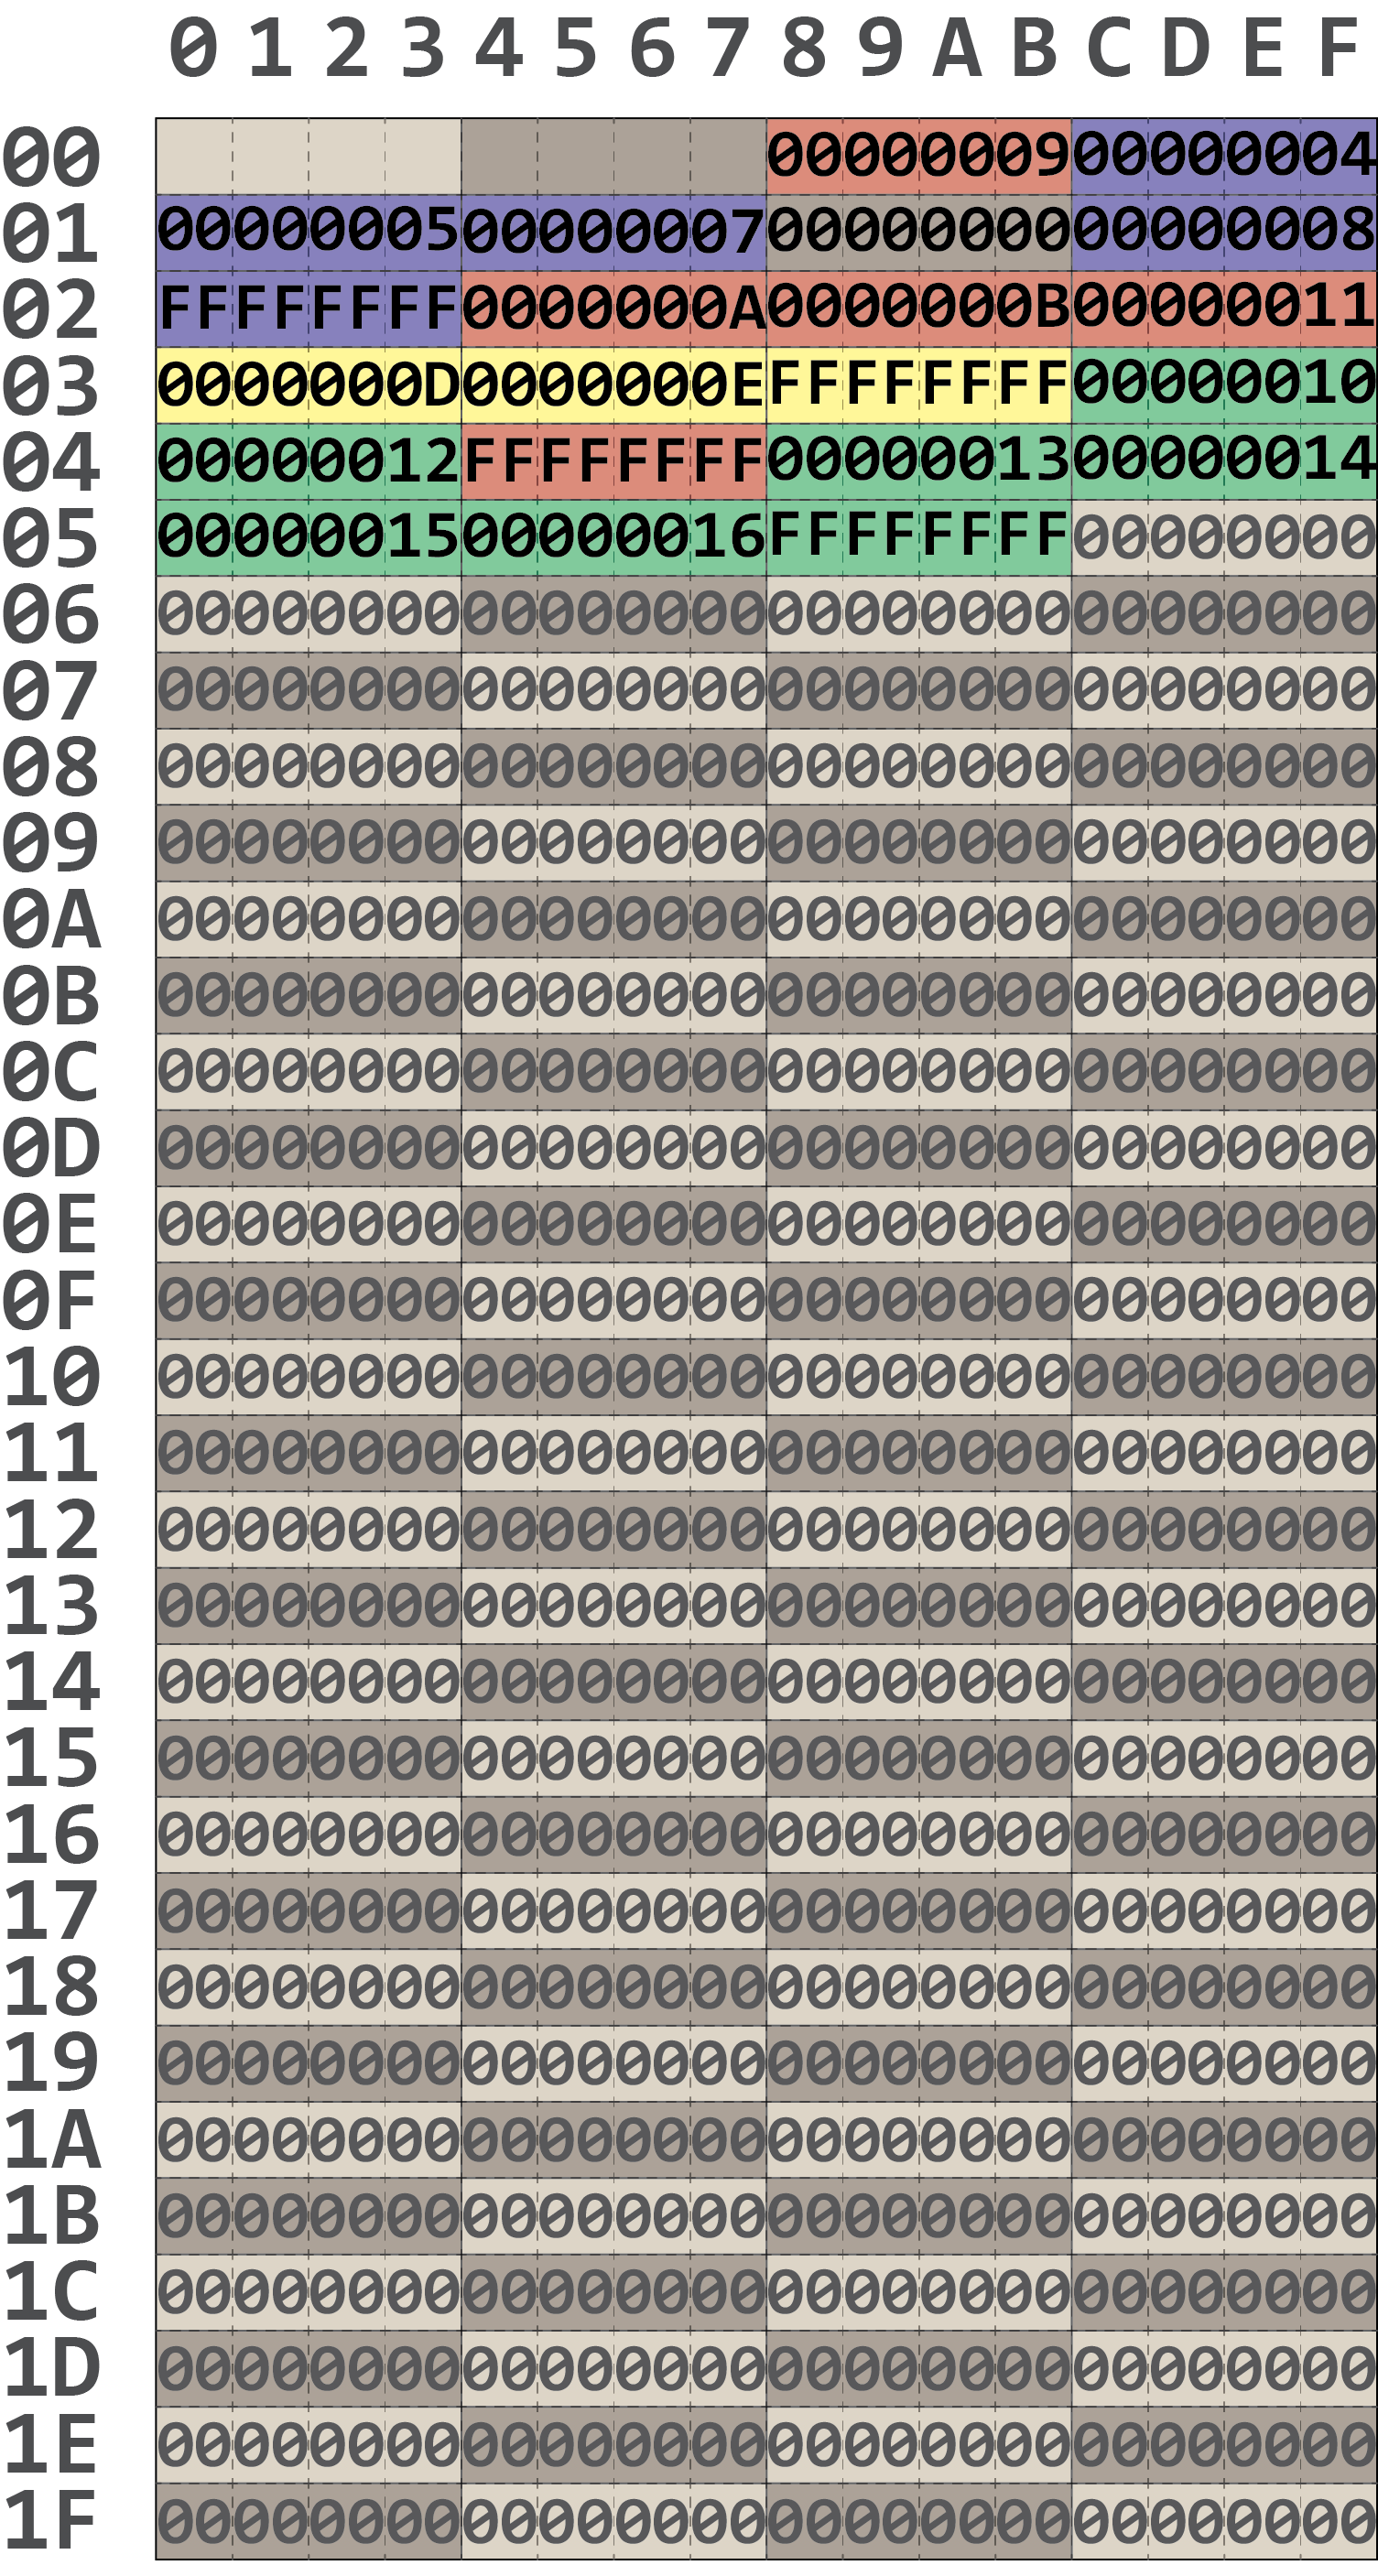
\includegraphics[width=0.95\textwidth]{img/fat32-voorbeeld.png}
        \caption{FAT sector.}
        \label{fig:fat-example}
    \end{subfigure}
    \caption{(a) Sector van een folder en (b) een sector van een FAT.}
\end{figure}

In \cref{fig:folder-cluster} staat een voorbeeld gegeven van een cluster welke behoort tot een folder. Dit cluster is opgedeeld in blokjes van 32 bytes waarbij elke blokje een omschrijving (metadata) bevat van een bestand of een subfolder. Of het stukje data een bestand of een folder beschrijft valt te bepalen aan de attribuutbyte. Het stukje metadata bevat ook een 32-bit clusteradres opgedeeld in een hoog 16-bit en een laag 16-bit fragment van dit adres. Tenslotte wordt ook de grootte van het bestand opgeslagen zodat bepaald kan worden hoeveel sectoren uitgelezen zouden moeten worden. 

Het clusteradres vormt echter enkel het eerste adres van een bestand of subfolder en een bestand of folder kan groter zijn dan een enkel cluster. In dat geval moet men weten welke clusters volgen na het eerste cluster. Dit is de functie van de FAT. De FAT geeft per cluster aan of er een vervolgcluster is. Als er geen vervolgcluster is, dan staat er in de FAT de waarde \pkb{0xFFFFFFFF}. Als er wel een vervolgcluster is, dan wordt het nummer van dit vervolgcluster genoemd. Vervolgens kan dit vervolgcluster ook weer een volgend cluster hebben en zo kunnen we dit proces blijven herhalen totdat er het adres \pkb{0xFFFFFFFF} gevonden wordt voor een cluster. Zie ter illustratie \cref{fig:fat-example}. Deze FAT geeft bijvoorbeeld aan (met de rode blokjes) dat er een bestand of cluster zich bevindt in de clusters \pkb{0x00000003}, \pkb{0x00000009}, \pkb{0x0000000A}, \pkb{0x0000000B} en tenslotte \pkb{0000011}; 5 clusters dus in totaal. Een ander voorbeeld betreft een bestand of folder aangegeven met de blauwe clusters. Dit bestand of folder omvat de clusters \pkb{0x00000003}, \pkb{0x00000004}, \pkb{0x00000005}, \pkb{0x00000007} en tenslotte \pkb{0x00000008}. Clusters met adres \pkb{0x00000000} zijn lege clusters welke nog opgevuld kunnen worden met data.

%
%
%
\section{CAS bestanden}
\label{sec:cas-files}

\pkb{.CAS} bestanden zijn een bestandsformaat bedacht in 1996\footnote{\url{https://www.komkon.org/~dekogel/m2000.html}} door Marcel de Kogel om programma's van \pkb{P2000T} cassettes op te slaan op een moderne(re) computer. Deze bestanden bestanden uit \textbf{blokken} van 1280 bytes (\pkb{0x500}) bytes. Elk \textbf{blok} van \pkb{0x500} bytes is weer opgedeeld in een header van \pkb{0x100} bytes en een data gedeelte van \pkb{0x400} bytes. Deze header is een kopie van het geheugen \pkb{0x6000 - 0x6100} tijdens het wegschrijven van de cartridge. Van dit stukje geheugen blijkt (achteraf) alleen het stukje \pkb{0x6040 - 0x605F} relevant voor de beschrijving van het \pkb{.CAS} bestand. In \cref{tab:cassette-metadata} staat een overzicht van de informatie die in dit geheugenblok opgenomen is.

\begin{table}
\caption{Omschrijving van de relevante data voor een cartridge in geheugenblok \pkb{0x6040 - 0x605F}.}
\label{tab:cassette-metadata}
\centering
\begin{tabular}{|r|l|}
\hline
Adres & Omschrijving \\
\hline
\pkb{0x6030-0x6031} & Transfer adres \\ \hline
\pkb{0x6032-0x6033} & Bestandsgrootte \\ \hline
\pkb{0x6034-0x6035} & Record grootte \\ \hline
\pkb{0x6036-0x603D} & Label (1/2) \\ \hline
\pkb{0x603E-0x6040} & Extensie \\ \hline
\pkb{0x6041-0x6042} & Type \\ \hline
\pkb{0x6043-0x6044} & Startadres \\ \hline
\pkb{0x6045-0x6046} & Load \\ \hline
\pkb{0x6047-0x604E} & Label (2/2) \\ \hline
\pkb{0x604F} & Aantal resterende blokken bij inlezen \\
\hline
\end{tabular}
\end{table}

%
%
%
\section{PRG bestanden}
\label{sec:prg-files}

\pkb{PRG} bestanden zijn speciale machinecode bestanden gemaakt voor de \product. Deze bestanden hebben een 16-byte header, worden op een vaste positie in het geheugen geplaatst en uitgevoerd met een nieuwe stack. De bestanden worden geplaatst op \pkb{0xA000-0xDCFF} en mogen maximaal \pkb{0x3D00} bytes lang zijn.\footnote{Ongeveer 15.25 KiB, net iets minder dan de grootte van een cartridge ROM, welke 16 KiB is.} De stack voor deze bestanden begint op \pkb{0xDEFF} en loopt afwaarts naar \pkb{0xDD00}, hetgeen een stackgrootte van 512 bytes geeft. Voor het draaien van \pkb{PRG} bestanden heeft men tenminste een 16 KiB geheugenuitbreiding nodig. Indien er enkel een 16 KiB geheugenuitbreiding aanwezig is (en niet meer) op de \pkb{P2000T}, dan zal de stack voor \pkb{BASIC} en het menu zich bevinden in \pkb{0xDF00-0xDFFF} waardoor dit stukje geheugen onaangetast moet blijven.

De header van de \pkb{PRG} bestanden is vergelijkbaar met de header voor \sleuf{1} cartridges. Het eerste karakter dient altijd een \pkb{0x50} te zijn, corresponderend met de ASCII waarde voor de hoofdletter \pkb{P}. Hierna volgen 2 x 16-bit waarden\footnote{In little-endian notatie, zie \cref{sec:endianness} op Pagina \pageref{sec:endianness}.}, corresponderend met het aantal bytes van het programma gevolgd door de CRC-16 checksum.\footnote{Zie \cref{sec:crc16-checksum} op Pagina \pageref{sec:crc16-checksum} voor meer informatie over CRC-16 checksums.} Deze CRC-16 checksum begint vanaf positie \pkb{0x10}, dus na de 16-byte header. Tenslotte resteren 11 karakters die de gebruiker vrij mag invullen, maar waarvan wordt aangeraden om een 8+3 bestandsnaam te gebruiken.

In tegenstelling tot \pkb{CAS} bestanden keren \pkb{PRG} bestanden wel terug naar het menu wanneer deze afgesloten worden. Om die reden is het programma opgeslagen in de \pkb{PRG} bestanden zelf verantwoordelijk voor het aanmaken en opruimen van de stack en het herpositioneren van de stackpointer \pkb{SP}. Middels de \pkb{Z88dk} toolchain is het echter vrij eenvoudig om dit op te stellen.